In the following, we write $C(e,e'),M(s,e),EN(s,e)$ to indicate variables
$C_{e,e'},M_{s,e},$ and $EN_{s,e}$ respectively.
\begin{example}
    Consider a firewall where we initially allow all outgoing packets and block all incoming packets.
    We want to allow incoming packets once a packet is sent outside.
    \begin{center}
        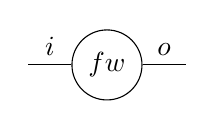
\begin{tikzpicture}[node distance={15mm},main/.style = {draw, circle}]
            \node[main] (s) {$fw$};
            \draw (s) -- node[above]{$i$} (-1,0);
            \draw (s) -- node[above]{$o$} (1,0);
        \end{tikzpicture}
    \end{center}
    We may represent this network with an event structure
    $\mathrm{E} = (\s{i,o},\e,\vdash)$ where events $o,i$ for incoming
    and outgoing packets respectively.
    We assume an empty conflict relation and enabling relation
    $\vdash$ the least one that satisfies:
    \begin{align*}
        \e \vdash i, \e \vdash o
    \end{align*}
    The functions of the causal model are as follows:
    \begin{align*}
        \f{M(\e,i)}     & = Min(\e,i) \wedge Con(\e) = Min(\e,i)   \\
                        & = \neg M(\s{o},i)                        \\
        \f{M(\e,o)}     & = Min(\e,o) \wedge Con(\e) =  Min(\e,o)  \\
                        & = \neg M(\s{i},o)                        \\
        \f{M(\s{i},o)}  & = \F                                     \\
        \f{M(\s{o},i)}  & = \F                                     \\
        \f{EN(\e,i)}    & = M(\e,i) \wedge Con(\e) = M(\e,i)       \\
        \f{EN(\e,o)}    & = M(\e,o) \wedge Con(\e) = M(\e,o)       \\
        \f{EN(\s{o},i)} & =
        \left( M(\s{o},i) \vee EN(\e,i)  \right) \wedge Con(\s{o}) \\
                        & = M(\s{o},i) \vee EN(\e,i)               \\
        \f{EN(\s{i},o)} & =
        \left( M(\s{i},o) \vee EN(\e,o) \right)
        \wedge Con(\s{i})                                          \\
                        & = M(\s{i},o) \vee EN(\e,o)
    \end{align*}
    This yields the following causal graph:
    \begin{center}
        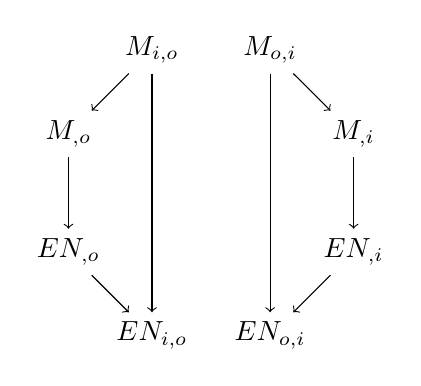
\begin{tikzpicture}[node distance=15mm]
            \node (moi) {$M_{\s{o},i}$};
            \node (mei) [below right of=moi] {$M_{\e,i}$};
            \node (eei) [below of=mei] {$EN_{\e,i}$};
            \node (eoi) [below left of=eei]{$EN_{\s{o},i}$};
            \draw[->] (moi) -- (mei);
            \draw[->] (mei) -- (eei);
            \draw[->] (eei) -- (eoi);
            \draw[->] (moi) -- (eoi);

            \node (mio) [left of=moi] {$M_{\s{i},o}$};
            \node (meo) [below left of=mio] {$M_{\e,o}$};
            \node (eeo) [below of=meo] {$EN_{\e,o}$};
            \node (eio) [below right of=eeo]{$EN_{\s{i},o}$};
            \draw[->] (mio) -- (meo);
            \draw[->] (meo) -- (eeo);
            \draw[->] (eeo) -- (eio);
            \draw[->] (mio) -- (eio);
        \end{tikzpicture}
    \end{center}
    Now let $\sigma = \s{o}$ be a counterexample.
    Assume that we want to declare $M(\s{i},o) = \F$ as a cause of
    $\sigma \in \mathcal{F}(\mathrm{E})$ using $(\e,\e,\T)$ as a witness.
    First, the AC1 condition is satisfied:
    \begin{align*}
        \m \vDash M(\s{i},o) = \F
        \wedge \vec V = \vec v
        \wedge \sigma \in \mathcal{F}(\mathrm{E})
    \end{align*}
    Next, we need to verify the AC2(a) condition:
    \begin{align*}
        \m \vDash [M(\s{i},o) \la T] \sigma \not \in \mathcal{F}(\vte)
        \wedge \vec v \in \mathcal{E}
    \end{align*}
    Assume that we set $M(\s{i},o)$ to true.
    $M(\e,o)$ depends on $M(\s{i},o)$, $E(\e,o)$ depends on $M(\e,o)$, and
    $E(\s{i},o)$ depends on both $M(\s{o},i)$ and $E(\e,i)$
    and these are the only variables that are affected by changing
    $M(\s{i},o)$.
    Thus we have:
    \begin{align*}
        \m & \vDash [M(\s{i},o)\la \T] M(\e,o) = \F     \\
        \m & \vDash [M(\s{i},o)\la \T] EN(\e,o) = \F    \\
        \m & \vDash [M(\s{i},o)\la \T] EN(\s{i},o) = \T
    \end{align*}
    Thus we have:
    \begin{align*}
        \m & \vDash [M(\s{i},o)\la \T]EN(\e,i) = \T    \\
        \m & \vDash [M(\s{i},o)\la \T]EN(\s{o},i) = \T \\
        \m & \vDash [M(\s{i},o)\la \T]EN(\e,o) = \F    \\
        \m & \vDash [M(\s{i},o)\la \T]EN(\s{i},o) = \T \\
        \m & \vDash [M(\s{i},o)\la \T]Con(i,o) = \F
    \end{align*}
    So, if $\mathrm{E}'' = \vte = (\s{i,o},\e, \vdash'')$
    after we have set $M(\s{i},o)$ to true we have:
    \begin{align*}
        \e \vdash'' i, \s{o} \vdash'' i, \s{i} \vdash '' o
    \end{align*}
    Thus configurations of the $\mathrm{E''}$ would be as the right figure
    below:
    \begin{center}
        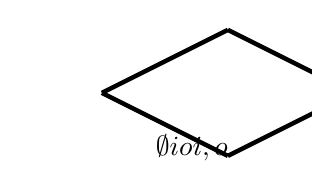
\begin{tikzpicture}[scale=0.8]
            \crd{0}{0}{$\emptyset$}
            \crd[left]{-2}{1}{$\s{i}$}
            \crd[right]{2}{1}{$\s{o}$}
            \crd[right]{0}{2}{$\s{i,o}$}
            \draw [ultra thick] (0,0) -- (2,1);
            \draw [ultra thick] (0,0) -- (-2,1);
            \draw [ultra thick] (-2,1) -- (0,2);
            \draw [ultra thick] (2,1) -- (0,2);
        \end{tikzpicture}
        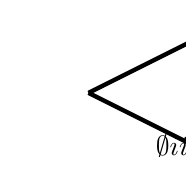
\begin{tikzpicture}[scale=0.8]
            \crd{0}{0}{$\emptyset$}
            \crd[left]{-2}{1}{$\s{i}$}
            \crd[right]{0}{2}{$\s{i,o}$}
            \draw [ultra thick] (0,0) -- (-2,1);
            \draw [ultra thick] (-2,1) -- (0,2);
        \end{tikzpicture}
    \end{center}
    We can easily verify that $\mathrm{E}''$ is an event structure.
    Now, since $\e \not \vdash'' o$, thus $\sigma$ is not a configuration
    of $\mathrm{E}''$.
    So the AC2(a) condition is also satisfied.
    Since we have used an empty $\vec W$ set for the witness, and AC2(a)
    condition is satisfied, thus we can conclude that $M(\s{i},o) = \F$ is a
    cause of $\sigma \in \mathcal{F}(\mathrm{\mathfrak{E}( \vec V)})$.
\end{example}

\begin{example}
    Consider the following network where wish to forward traffic from $a$ and $b$ to $c$, while limiting the traffic on the link 3 so that
    at any moment there must be at most one packet traversing this link.
    \begin{center}
        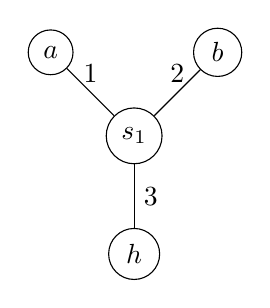
\begin{tikzpicture}[node distance={15mm},main/.style = {draw, circle}]
            \node[main] (s) {$s_1$};
            \node[main] (h) [below of=s] {$h$};
            \node[main] (a) [above left of=s]{$a$};
            \node[main] (b) [above right of=s]{$b$};
            \draw (a) --  node[above]{1}(s);
            \draw (b) --  node[above]{2}(s);
            \draw (s) --  node[right]{3}(h);
        \end{tikzpicture}
    \end{center}
    We define events $a,b$ representing the forwarding of a packet from
    1 to 3 and 2 to 3 respectively.
    We define an event $c$ when congestion is detected on link 3 (at least two packets are being traversed through the link).
    For this network, we can define an event structure $\mathrm{E}$
    with an empty conflict relation and an enabling relation the least
    one for which we have:
    \begin{align*}
        \e \vdash a, \e \vdash b, \s{a,b} \vdash c
    \end{align*}
    Which has configurations of the form:
    \begin{center}
        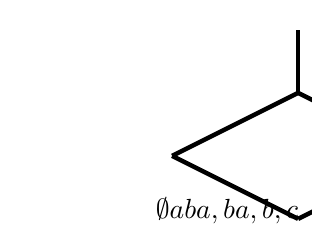
\begin{tikzpicture}[scale=0.8]
            \crd{0}{0}{$\emptyset$}
            \crd[above]{-2}{1}{$\s{a}$}
            \crd[above]{2}{1}{$\s{b}$}
            \crd[left]{0}{2}{$\s{a,b}$}
            \crd[left]{0}{3}{$\s{a,b,c}$}
            \draw [ultra thick] (0,0) -- (-2,1);
            \draw [ultra thick] (0,0) -- (2,1);
            \draw [ultra thick] (-2,1) -- (0,2);
            \draw [ultra thick] (2,1) -- (0,2);
            \draw [ultra thick] (0,2) -- (0,3);
        \end{tikzpicture}
    \end{center}
    In the causal model we have:
    \begin{align*}
        \f{M(\e,a)}       & = Min(\e,a)                              \\
                          & = \neg M(\s{b},a) \wedge \neg M(\s{c},a)
        \wedge \neg M(\s{b,c},a)                                     \\
        \f{M(\e,b)}       & = Min(\e,b)                              \\
                          & = \neg M(\s{a},b) \wedge \neg M(\s{c},b)
        \wedge \neg M(\s{a,c},b)                                     \\
        \f{M(\s{a,b},c)}  & = Min(\s{a,b},c) \wedge Con(\s{a,b})     \\
                          & = \neg M(\e,c) \wedge \neg M(\s{a},c)
        \wedge \neg M(\s{b},c) \wedge Con(\s{a,b})                   \\
        \f{EN(\e,a)}      & = M(\e,a)                                \\
        \f{EN(\s{b},a)}   & = M(\s{b},a) \vee EN(\e,a)               \\
        \f{EN(\s{c},a)}   & = M(\s{c},a) \vee EN(\e,a)               \\
        \f{EN(\s{b,c},a)} & = (M(\s{b,c},a) \vee EN(\e,a) \vee
        EN(\s{b},a) \vee EN(\s{c},a) ) \wedge Con(\s{b,c})           \\
        \f{EN(\e,b)}      & = M(\e,b)                                \\
        \f{EN(\s{a},b)}   & = M(\s{a},b) \vee EN(\e,b)               \\
        \f{EN(\s{c},b)}   & = M(\s{c},b) \vee EN(\e,b)               \\
        \f{EN(\s{a,c},b)} & = (M(\s{a,c},b) \vee EN(\e,b) \vee
        EN(\s{a},b) \vee EN(\s{c},b) ) \wedge Con(\s{a,c})           \\
        \f{EN(\e,c)}      & = M(\e,c)                                \\
        \f{EN(\s{a},c)}   & = M(\s{a},c) \vee EN(\e,c)               \\
        \f{EN(\s{b},c)}   & = M(\s{b},c) \vee EN(\e,c)               \\
        \f{EN(\s{a,b},c)} & = (M(\s{a,b},c) \vee EN(\e,c) \vee
        EN(\s{a},c) \vee EN(\s{b},c) ) \wedge Con(\s{a,b})           \\
    \end{align*}
    All other functions are constantly false.

    \begin{center}
        \begin{tikzpicture}[node distance=20mm]
            \node (mea) {$M(\e,a)$};
            \node (mbca) [above of=mea] {$M(\s{b,c},a)$};
            \node (cbc) [above=5mm of mbca] {$C(b,c)$};
            \node (mba) [above left of=mea] {$M(\s{b},a)$};
            \node (mca) [above right of=mea] {$M(\s{c},a)$};
            \node (eea) [below=5mm of mea] {$EN(\e,a)$};
            \node (eba) [below left of=eea] {$EN(\s{b},a)$};
            \node (eca) [below right of=eea] {$EN(\s{c},a)$};
            \node (ebca) [below right of=eba] {$EN(\s{b,c},a)$};
            \draw[->] (mbca) -- (mea);
            \draw[->] (mba) -- (mea);
            \draw[->] (mba) -- (eba);
            \draw[->] (mca) -- (mea);
            \draw[->] (mca) -- (eca);
            \draw[->] (mea) -- (eea);
            \draw[->] (eea) -- (eba);
            \draw[->] (eea) -- (eca);
            \draw[->] (eea) -- (ebca);
            \draw[->] (eba) -- (ebca);
            \draw[->] (eca) -- (ebca);
            \draw[->] (cbc) edge (mbca);
            \draw (mbca) -- (-3,2);
            \draw (-3,2) -- (-3,-3.9);
            \draw [->] (-3,-3.9) -- (ebca);
            \draw (cbc) -- (3,3.1);
            \draw (3,3.1) -- (3,-3.9);
            \draw [->] (3,-3.9) to (ebca);
        \end{tikzpicture}
    \end{center}

    Obviously, $\sigma$ is a configuration of $\mathrm{E}$.
    Now, let's consider $C(a,x) = \F$ as a cause using the witness
    $(\e,\e,\T)$.
    Now let $\mathrm{E}'' = \vte = (E, \#'',\vdash'')$ after we set $C(a,x)$ to true. So we have $a\#''x$ and $x\#''a$.
    First, note that $C(a,x)$ only affects terms like $Con(s)$
    where $ \s{a,x} \subseteq s$ which in turn only affects
    variables of the form $M(s,e)$ or $EN(s,e)$.
    So, we can safely conclude that changing $C(a,x)$ has no effect
    on $M_{\e,a},M_{\e,x},M_{\s{a},b},M_{\s{b},a}$ as well as
    $EN_{\e,a},EN_{\e,x},EN_{\s{a},b},EN_{\s{b},a}$.
    Thus we have:
    \begin{align*}
        \e \vdash'' a,
        \e \vdash'' x,
        \s{a} \vdash'' b,
        \s{x} \vdash'' y \\
        a\#''y,y\#''a,x\#''b,b\#''x,a\#''x, x\#''a
    \end{align*}
    So, the configurations of $\mathrm{E}''$ have the form:
    \begin{center}
        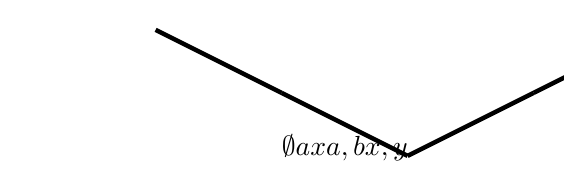
\begin{tikzpicture}[scale=0.8]
            \crd{0}{0}{$\emptyset$}
            \crd[above]{-2}{1}{$\s{a}$}
            \crd[above]{2}{1}{$\s{x}$}
            \crd[left]{-4}{2}{$\s{a,b}$}
            \crd[left]{4}{2}{$\s{x,y}$}
            \draw [ultra thick] (0,0) -- (-2,1);
            \draw [ultra thick] (0,0) -- (2,1);
            \draw [ultra thick] (-2,1) -- (-4,2);
            \draw [ultra thick] (2,1) -- (4,2);
        \end{tikzpicture}
    \end{center}
    In the new event structure, $\sigma$ is no longer a configuration, thus $AC2(a)$ is satisfied.
    Since we have used an empty $\vec W$ in the witness and AC1 and AC2(a)
    are satisfied, thus we can conclude that $C(a,x) = \F$ is a cause of
    $\sigma \in \mathcal{F}(\mathrm{E}')$


\end{example}

\begin{example}
    Consider the following network where we want to implement a firewall
    on the switch $s$.
    The goal of the firewall is to simply block all incoming packets.
    We define two events $a$ and $b$ representing the arrival of a packet
    on the switch from the hosts $a$ and $b$ respectively.
    Assume that switch forwards all packets it received.
    We use an event $i$ to represent the forwarding of an arbitrary packet
    to $i$.
    So, we can represent this setting with an event structure $\mathrm{E}$
    with events $\s{a,b,i}$, an empty conflict relation and enabling relation
    the least one that satisfies:
    \begin{align*}
        \e \vdash a, \e \vdash b, \s{a} \vdash i, \s{b} \vdash i
    \end{align*}
    
    \begin{center}
        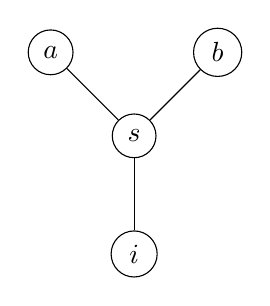
\begin{tikzpicture}[node distance={15mm},main/.style = {draw, circle}]
            \node[main] (s) {$s$};
            \node[main] (a) [above left of=s] {$a$};
            \node[main] (b) [above right of=s] {$b$};
            \node[main] (i) [below of=s] {$i$};
            \draw (s) -- (a);
            \draw (s) -- (b);
            \draw (s) -- (i);
        \end{tikzpicture}
    \end{center}
    We define an event structure where
    $\mathcal{E} = \s{a,b,c,i}$.
    We let $a,b,c$ to represent the events of sending
    a packet from $a$,$b$ and $c$ to $s$ respectively.
    Let $i$ indicate the event of the forwarding of
    an arbitrary packet from $s$ to $a$ (this may coming
    from either $b$ or $c$).
    We consider an empty conflict relation and enabling
    relation the least one for which we have:
    \begin{align*}
        \e \vdash a,\e \vdash b, \e \vdash c,
        \s{b} \vdash i, \s{c} \vdash i
    \end{align*}
    We may consider the configuration $\sigma = \s{b,c,i}$ as a
    counterexample since $i$ is happened while $a$ has not been happened yet.
\end{example}